\documentclass{IEEEtran}
%\usepackage{latex8}
\usepackage{times}
\usepackage{algorithm}
\usepackage{algorithmic}
\usepackage{graphicx}
\usepackage{epsfig}
\usepackage{color}
\usepackage{amssymb}
\usepackage{flushend}
\usepackage{cite,float}

\newtheorem{theorem}{Theorem}[section]
\newtheorem{lemma}[theorem]{Lemma}
\newtheorem{proposition}[theorem]{Proposition}
\newtheorem{corollary}[theorem]{Corollary}

\newenvironment{definition}[1][Definition]{\begin{trivlist}
\item[\hskip \labelsep {\bfseries #1}]}{\end{trivlist}}
\newenvironment{example}[1][Example]{\begin{trivlist}
\item[\hskip \labelsep {\bfseries #1}]}{\end{trivlist}}
\newenvironment{remark}[1][Remark]{\begin{trivlist}
\item[\hskip \labelsep {\bfseries #1}]}{\end{trivlist}}

\begin{document}

\title{Participatory Privacy via Anonymous Network Protocols}


\numberofauthors{2}

\author{
\alignauthor Chih-Jye Wang\\
      \affaddr{Dept. of Computer Science and Software Engineering}\\
      \affaddr{Auburn University}\\
     \affaddr{Auburn, AL 36849, USA}\\
      \email{wangchj@auburn.edu}
\alignauthor Wei-Shinn Ku\\
       \affaddr{Dept. of Computer Science and Software Engineering}\\
       \affaddr{Auburn University}\\
      \affaddr{Auburn, AL 36849, USA}\\
       \email{weishinn@auburn.edu}
}


%\conferenceinfo{ACM GIS'09,} {November 4-6, 2009. Seattle, WA, USA}
%\CopyrightYear{2010} \crdata{ISBN 978-1-60558-649-6/09/11}


\maketitle

\begin{abstract}
In the participatory sensing, users with mobile devices (e.g. cell phones
and laptop computers) participate in the collection of environmental
information around them and submit the collected data to a central server
for processing and analysis. Identity privacy of mobile users in this model
is a major concern that hinders the adoption of this computing model. In
this paper, we propose an anonymous networking protocol approach to protect
the identity of participants of such computing model.
\end{abstract}

%\category{H.2.8}{Database Management}{Database Application}[spatial databases and GIS]

%\terms{Algorithms and Experimentation}

%\keywords{Location-based services, location privacy and spatial cloaking} % NOT required for Proceedings

\section{Introduction}\label{sec-intro}
In the participatory sensing, users with mobile devices
(e.g. cell phones and GPS devices) participate in the collection of environmental
information around them and submit the collected data to a central server
for processing, analysis, and storage\cite{DBLP:conf/mobisys/MunRSYBEHHWB09}.
An example is the OpenStreetMap\cite{DBLP:journals/pervasive/HaklayW08}
project which collects user contributed GIS
data (such as GPS traces and POIs) and constructs an online map, from mobile
data, open for anyone to use. 
Other examples of participatory sensing
include cooperative collection of gas prices \cite{DBLP:conf/dcoss/DongKCB08},
monitoring of traffic conditions \cite{DBLP:conf/dcoss/ConceicaoFB08}, and
photo sharing through mobile applications such as Facebook and Instagram.

This model of "crowd" data collection has many advantages due to that the
dynamic environmental data and information are quickly captured by mobile
users and disseminated to other users or to central servers for analysis.
Government censoring of information captured and distributed is also less
effective in this model since there could be many mobile devices that are
capturing the same event.

Despite the advantages, privacy of the users who contribute is a major
issue in participatory sensing and crowd-sourcing. Users may not want to
leak their locations with the contributed data lest their movement being
tracked. In the case of controversial photos, a user may not want to
reveal his or her identity to the server (such as
Instagram\footnote{http://instagr.am/}) that collect
the data since the user's identity may be saved on the server and later
uncovered by government entities for prosecution. It is a fact that
services on the web collect user identifications along with the data
submitted by their users\cite{wiki_privacy}. Even with websites, such as
Wikipedia\footnote{http://www.wikipedia.com} and
4chan\footnote{http://www.4chan.org/faq\#what4chan}, that advise to be
anonymous log IP address of contributors. With
an IP address (and if IP uniquely identify a user), a piece of
information stored on a server (be it a photo, or a file) can be traced
back to a user thus compromise the user's privacy.

How to guarantee that a server will not gather users identification when
a service advertise it? In this paper, we focus on the problem of keeping
user's identity private
in participatory sensing and crowd-sourcing environment. We want to keep
a request to a server anonymous to all entities in a network including
the server itself (since we know they log user activities).
We study a way to
minimize the probability of identifying and linking a piece of data
in a computer network to a user.
Then we propose a way to protect the identity of participants
of such computing model by using an anonymous networking protocol.
The goal of the protocol is to remove the source information from the data
packet. We call this One-Way Protocol since the source information is
completely removed, and the server is unable to reply any kind of
acknowledgement back to the client. The protocol will be implemented on
both the server and the client to achieve the anonymous effect.

%In Section 2, we propose a fundamental theoretical novel One-Way protocol
%that probably has no practical usefulness except to demonstrate the idea.
%(In Section X we present other solutions to this problem). In section 3
%we refine the theoretical protocol so that it can be architectures on
%existing networking infrastructures and technologies. Validation and data
%integrity is covered in section 4. 
\section{Related Works}\label{sec-related-works}
One of the earliest work on anonymous communication is on untraceable
electronic mail by Chaum\cite{DBLP:journals/cacm/Chaum81}. The work proposed
a way of sending an electronic mail to a receiver in which the sender
remain anonymous using one or a series of proxy computers called Mixes.
Chaum's solution relies heavily on public key cryptography in a way that
before forwarding a mail to a mix, the message and the receiver's address
is encrypted using the mix's public key. Upon receiving an electronic
message, the mix extracts the information
and forwards the mail to the intended receiver. In the case of multiple
mixes, the sender performs one public key cryptography for each mixes before
sending a mail to the first mix. The mix then forward it to the next mix
and so on until the mail reaches the receiver. One of the drawback of the
solution proposed in \cite{DBLP:journals/cacm/Chaum81} is scalability since
the senders depend on fixed proxies and if there are not proxies, the
solution will not work. Also multiple public key cryptography is expensive
for mobile devices. Multiple public key is acceptable for small file, but
for large files that need to be broken down and sent with multiple segments,
multiple encryption may not be acceptable.

Another well known research of sender anonymity is the
onion routing\cite{DBLP:conf/uss/DingledineMS04}. The onion routing
follows the similar approach as in \cite{DBLP:journals/cacm/Chaum81} of
using multiple proxies and multiple encryptions. Before sending a file,
the sender selects a number of proxies called onion routers. The selected
routers have no say in the selection process, thus mitigating malicious
node collaboration attack. After selecting the routers, the sender
encrypts its data with the key of the first router, then encrypt the result
of that with the key of the second router, and does the same for all the
routers. Onion routing is robust in terms
of security and can be used in many applications, but it has the same
drawback as in Chaum's approach that it is computationally expensive
because of the multiple encryptions. Our solution does not impose multiple
encryption to the application, but give that choice to the developer
of the application.

Freenet, a distributed anonymous storage system was proposed
in \cite{DBLP:conf/diau/ClarkeSWH00}. The goal of the system is to utilize
the peers in the network for storage and at the same time achieving anonymity
of the author of the files. Freenet utilizes file keys obtained by public
key cryptography and hashing to achieve efficient file storage and searching.
In order to achieve author anonymity, a node on the Freenet sends a file
to a peer, and the peer forwards the file to another peer and so on, much
like the solution in Crowds. Although, the system pertains to file storage,
the technique of utilizing peers to hide the identity of the originator of
a file is useful in our scenario and we take a similar approach with our
data verification of our design.

Crowds\cite{DBLP:journals/cacm/ReiterR99} utilizes peer-to-peer network
to blend the sender into a large number of users (a crowd) so that the
receiver does not know the true identity of the sender.
To send a file, the sender joins a close-by crowd and sends the file to
one of its peers in the crowd called jondo (a short name for John Doe).
When a peer receives a send request, it decides whether to forward the
data to another peer based on the variable $p_f$ that determines the
probability of forwarding the packet.

The closest work to ours is research on privacy for mobile users in sensing
networks \cite{DBLP:conf/percom/HuS10} by Hu and Shahabi. The assumption of the
work is that data collection service providers often log the identity of the
user with the file they submit. The disclosure of this sensitive information
leads to the compromising of user privacy. The solution is to leverage
social network to forward a file to multiple peers before sending it to
the server. Large consumption of network bandwidth is a big disadvantage in
this approach since a file is sent to multiple users, and this concern is
exacerbated in wireless mobile environments where bandwidth is limited.
In our approach, we do not forward the payload of the data to multiple peers,
only the control messages of the data transmission and saves tremendous amount
of bandwidth.
\section{Anonymous Protocol}\label{sec-protocol}

\begin{figure}[h]
\begin{center}
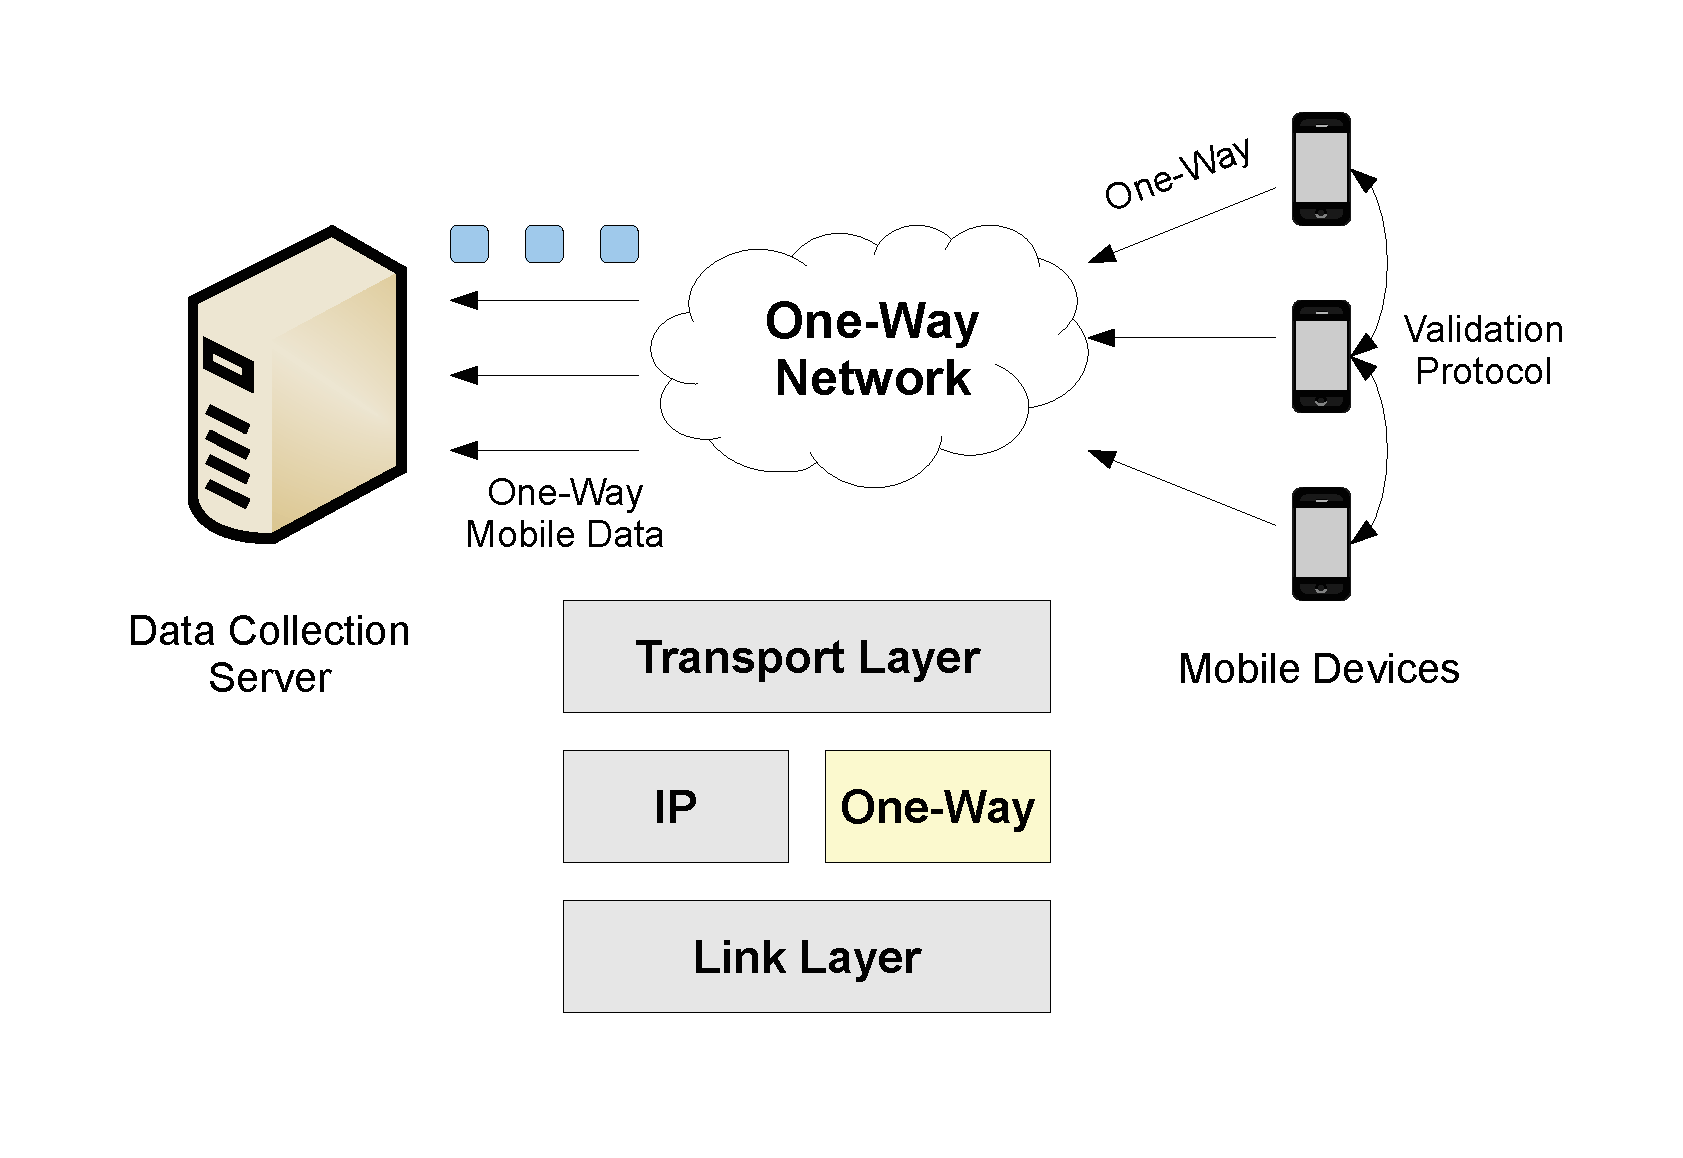
\includegraphics[width=3in]{figure1.eps}
\caption{\small \sl Anonymous Protocol.\label{fig:Stupendous}}
\end{center}
\end{figure}

\subsection{Overview}\label{proto-overview}
In this section, we describe our anonymous One-Way protocol, which completely
removes the ownership and
source information from the data transmitted to the data collection server.
Figure 1 illustrates the concept of the theoretical anonymous One-Way
protocol. One-Way is a packet routing protocol similar to the IP protocol.
Data are transmitted in packets. Each packet contains the address of the destination
host so that the packet can be correctly routed. One major difference between
One-Way protocol and other routing protocol is that, each packet does not
include the routing address of the sender (thus called One-Way). The source
address is intentionally removed so that the receiver of the data does not
know the identity of the sender. In other
words, contractually, the client does not include the source address and the
server will have no access to the source information and thus keeping the
client's identity private.

Our protocol is analogous to sending a parcel through a postal service without
sender's identity and address. An example is sending a hint to the police
pertaining a crime without revealing the sender's identity.

Unlike many other anonymous routing protocols, our protocol does not involve other
peers or mobile devices to transmit the data payload. This is particular helpful
in mobile environment in which bandwidth is limited. Some privacy aware protocols
first transmit the data payload to several mobile peers several times to mask
the identity of the sender before one of the random peers transmit the data to
the server. This puts tremendous bandwidth strain on the peers.

One drawback of a protocol without sender address is that the sender is unable
to get a feedback from the receiver whether a packet has been received (or
lost in transmission). To solve this problem, One-Way utilize a peer-to-peer
approach to verify correct transmission of a packet, much like the way
Crowds\cite{DBLP:journals/tissec/ReiterR98} uses to send data to a server.

For the validation, we want to construct a peer-to-peer network containing
$h$ nodes, where $h$ denotes the total number of hop counts for control
messages pass though. A peer node is denoted by $n_i$, meaning the
$i$th hop along the route. The peer network is a collection of nodes as
in Equation~\ref{eq:nodes}

\begin{equation}\label{eq:nodes}
\{n_0, n_1, ..., n_h\}
\end{equation}

We use $n_0$ to denote the originator of the data, and $n_h$ the last hop
that forward the data to the final receiver. For control messages travel
in the direction from sender to receiver, a node $n_i$ forwards the message
to its successor, such that $n_i \rightarrow n_{i+1}$. Similarly, for
control messages travel from the receiver back to the sender, a node 
forwards the messages to its predecessor, such that
$n_{i} \rightarrow n_{i-1}$. Table~\ref{tab:notations} summarizes the
notations used in this paper.

\begin{table}[h]
\centering
\caption{Summary of Notations} \label{tab:notations}
\begin{tabular}{c|l}
\hline
{\bf Notation} & {\bf Description}\\
\hline
$n_0$, $n_1$ ... & Peer nodes\\
$h$ & Total hop count\\
$I_s$, $I_r$ & Connection identifiers from sender and receiver, respectively\\
$A_i$, $A_r$ & Address of $i$th node and receiver, respectively\\
$D$ & Data payload\\
$s_i$ & $i$th sequence number; $s_0$ being initial sequence number\\
$c$ & Connection control message\\
$a$ & Acceptance control message\\
$p$ & Data payload message\\
$k$ & Acknowledgement control message\\
\hline
\end{tabular}
\end{table}

Opponents may argue that since the protocol resides on network layer (layer 3),
the source address could still be contained in the lower layer, e.g. the link
layer (layer 2). We argue that the source link address is different for
each hop on the route, and a route could easily contain 20 hops; therefore
the probability of tracing the link layer packet back to the original host is
really low.

\subsection{Anonymous Connection}\label{anonymous_connection}

Before transmitting data to a data collection server (receiver), the
sender makes an anonymous connection request to the server. The purpose
of the connection request is to establish a peer based route on which
acknowledgement of data transmission can be sent.

The sender initiates a connection by constructing an anonymous
connection request message, $c$. A request message contains the 
connection identifer $I_s$, routing
address (or identification), $A_r$, of the receiver,initial sequence
number $s_0$, and a hop count,
$h$. The structure of the request is defined in
Equation~\ref{eq:con_req_format}

\begin{equation}\label{eq:con_req_format}
c = \{I_s, A_r, s_0, h\}, h~\epsilon~\mathbb{N}_{\leq1}
\end{equation}

In the connection request packet, $h$ is a random natural number
denoting the number of peers the request should be forwarded to
before the request is sent to the server. The connection identifier $I_s$
is randomly generated and only last for the session and does not identify
a host.

After the sender has constructed the connection request message,
it sends the message to one of its peers running the protocol. When the
peer receives the request, it decrement the hop count $h$ by 1. If
the hop count reaches 0, then the peer sends the request to the server;
else, the peer forwards the request to another one of its peers. Note
a peer does not have to be a pure peer, but a node in the system whose
job is to facilitate communications for user nodes. Each peer in the
route keep track of the peer before and after for each request in order
to maintain the route information. If a peer declines a $c$ message,
the peer finds another peer. At the end of connection phase, the
peer-to-peer route should be constructed such that

\begin{equation}
sender(n_0) \rightarrow n_1 \rightarrow ... \rightarrow n_h \rightarrow receiver
\end{equation}

When the server receives the connection request, it sends back an acceptance
message $a$ to the node from which it receives the connection request ($n_h$).
The acceptance message contains a connection token $I_r$, as well as the
request identifier from the sender, $I_s$. The format of the acceptance
message is defined in Equation~\ref{eq:con_accept_format}

\begin{equation}\label{eq:con_accept_format}
a = \{I_r, I_s\}
\end{equation}

The node that receives the acceptance message from the receiver forwards
the message in reverse to the peer who forwarded the request message.
Each peer in the route keeps the route information based on $I_s$ and
the acceptance messages travels in revers on the same route until the
message reaches the original sender.

%[Discussion of the security of this connection approach]

%[Briefly describe routing table format and management for example, there
%is no activity for a connection for a long time. What should be done?]
\subsection{Payload Transmission}

Payload is the actual data transmitted to the server. In participatory
sensing, this is the data collected by the mobile devices from the
environment and include sensor data, photos, and videos. Payload
transmission does not involve peers since peer-forwarding in wireless
mobile environment is expensive; instead, payloads are transmitted
through the One-Way network, in which the packets only contain receiver
address and identification.

The payload transmission begins when the sender receives the acceptance
message from the server. In addition to the payload $D$, a payload
packet, denoted with $p$, also contains the address of of the receiver
$A_r$, the connection identifier $I_r$, and a sequence number $s$. The
format is defined in Equation~\ref{eq:payload_format}.

\begin{equation}\label{eq:payload_format}
p = \{A_r, I_r, s, D\}
\end{equation}

$I_r$ is the identifier issued by the server received from the connection
acceptance message. The purpose of this identifier is for the server to identify
a particular data transmission. For example, the server could be receiving
several data transmission simultaneously from different client each transmit
a file. The server assigns an identifier $I_r$ to each transmission to
differentiate the packets for the different transmissions. This field is
analogous to the port numbers in transport layers such as TCP and UDP to
multiplex packets for different connections and applications.

The sequence number $s$ in a payload packet identifies individual packets
for a transmission. The sequence numbers provide the order of the packets
and allow the receiver to identify if a packet is lost in the network, or
if packets arrived out of order.

The purpose of the connection establishment step before payload transmission
is to establish a channel in which the mobile client can verify that a packet
has been successfully received by the server. Techniques of reliable data
transfer in unreliable channel is out of scope of this paper. Reliable data
transfer mechanisms employed in TCP\cite{RFC793} and theoretical techniques
such as GO-Back-N and Select Repeat\cite{book:Kurose} can be employed with
our design. When the server wants to send a status of a packet back to
the client, it sends the status message through the peer-to-peer channel
established during connection establishment. In other words, after receiving
a payload packet $p$, the server sends an acknowledgement message, $k$, to the
node from which it received the connection request (also the node to which
it sends the connect acceptance message). Since all nodes on the anonymous route
remembers the previous node based on the connection identifiers, $I_s$ and
$I_r$, each node forwards $k$ to its previous peer until the message
reaches the originator of $p$.

%\begin{figure}[h]
%\begin{center}
%\includegraphics[width=3in]{arch.eps}
%\caption{\small \sl System Architecture.\label{fig:Stupendous}}
%\end{center}
%\end{figure}

\subsection{Node Disconnection and Failure}

When a node can no longer service a route for a connection due to
resource constraint or node shutting down, the disconnecting node (denoted
by $n_d$)
should notify its neighboring nodes of such event so that the interruption
of a connection and of delivering of control messages can be minimized.
In this section, we focus on disconnecting a single connection (as in
the case of resource constraint). If a node wishes to disconnect all
connections it supports (as in the case of node shut down), the $n_d$
performs a disconnection process discussed in this section for each
connection.

There are two scenarios for the $n_d$: the next node is an intermediate node,
and the $n_d$ is the last node in the route ($d$ = $h$).
For the first case in which the the $n_d$ is an intermediate node and the
next node is also an intermediate node, the $n_d$ should simply bridge the
gap and drop off from the route. In this case, the $n_d$ sends the node before
$n_{d-1}$
and after $n_{d+1}$
it a disconnection message containing the identity (the address)
of the two nodes. Once the connection between the two nodes has been
established, $n_d$ can remove the route information for the connection
from its routing table.

In the second case, the $n_d$ is the last node of the route and
communicates directly with the server. In this case, we do not want
just bridge the two nodes $n_{d-1}$ and $n_{d+1}$ since $n_{d-1}$
could be the originator of the data. In order to establish a new route
for the connection, $n_d$ sends a disconnection message to and telling
the server that a new control message route will be constructed for this
connection. $n_d$ also sends a route discovery message to $n_{d-1}$
and telling the node to construct a new route to the server. $n_{d-1}$
follows the same steps described in section~\ref{anonymous_connection}
to establish a new connection the the server. The connection algorithm
is detailed in Algorithm~\ref{alg:disconnect}.

\begin{algorithm}
\algsetup{linenosize=\small,linenodelimiter=. }
\caption{disconnect($n_d$)} \label{alg:disconnect}
\begin{algorithmic}[1]
\IF{$A_d$ = $A_r$}
    \STATE $m_1$ = DisconnectMessage($I_s$, $I_r$)
    \STATE $m_2$ = RediscoveryMessage($I_s$, $I_r$)
    \STATE SendToNode($A_r$, $m_1$)
    \STATE SendToNode($A_{d-1}$, $m_2$)
\ELSE
    \STATE $m_1$ = BridgeMessage($Forward$, $A_{d+1}$, $I_s$, $I_r$)
    \STATE $m_2$ = BridgeMessage($Backward$, $A_{d-1}$, $I_s$, $I_r$)
    \STATE SendToNode($A_{d-1}$, $m_1$)
    \STATE SendToNode($A_{d+1}$, $m_2$)
\ENDIF
\end{algorithmic}
\end{algorithm}

In the event of unforseen failure of a node, such as power or network
failure, the disconnected node $n_d$ is unable to notify its neighbors on
a route before disconnecting. When this happens the first thing that the
sender will notice is that it no longer receives acknowledgement message
of received packet from the server. To test for node failure in the path,
the sender $n_0$ can send a route test message into the route. When a
node $n_m$ receives the test message, it sends an acknowledgement back to
its predecessor $n_{m-1}$ on the route and forwards the test message to
its successor $n_{m+1}$ on the route. If an intermediate node on the route
$n_f$ cannot be contacted or does not acknowledge the test message, then
its predecessor $n_{f-1}$ sends a failure notice backward through the route
to notify the sender a failure has been detected. $n_{f-1}$ uses route
discovery algorithm to discovery a new route from $n_{f-1}$ to the server
and notify the new route has been successfully established. In the case
that there is no failure detected, but the sender still does not receive
acknowledgements from the server, the sender can select to terminate the
data transmission and peer connection.

\subsection{Connection Tear-Down}

After the entire file has been sent to and received by the server, the
sender can choose to tear down the connection so that the nodes can free
the resources used for the connection. To terminate a connection, the
sender injects the termination message identified by $I_s$ and $I_r$ into
the connection. Upon receiving the termination message, a node forwards
the message to its successor and free any resource associated with the
connection. Eventually the termination message reaches the server, and the
server frees the resource, and stores the received file.

\section{Attack Models}

In this section we consider several attack models and discuss how our
design offer protection against these attacks.

\subsection{Server Attack}
The first attack model is server attack. In this attack, the server cannot
be trusted or can be a source of identity of disclosure. Most services logs
the identity of the users with the data submitted through their services.
If the server is malicious, or mandated by someone powerful for disclosure,
privacy of the users are compromised.

First we analyze the payload transmission part of our design against
server attack. We assume that the server can see the packets sent to it,
but does not see the packets in the network before it reaches it. In
other words the server does not control the Internet and cannot perform
traffic analysis on the Internet. Under this assumption, in our One-Way
protocol the sender has the anonymity level of beyond suspicion since
a server cannot infer any identity information from the data packet it
receives. The only linking information is the identity of the network
device (e.g. link layer switch) at the last hop of the route. We assume
the service does not control the Internet, therefore it cannot link
this information back to the sender.

Next we analyze our validation protocol again server attack. Keep in mind,
our validation uses peer network to transmit acknowledgement and control
messages.
Since the server has to run our anonymous validation protocol, it is
consider one of the network peers and therefore it can
find out the users in the peer network, but the server does not know the
original hop count $h$ of the control packets. In addition, any peer can
potentially be connected with any other peers therefore, the sender is
also beyond suspicion in this case.

\subsection{Eavesdrop and Traffic Analysis}

In eavesdrop attack, we assume that the data transmission route is divided
into segments each controlled by a network administrator. An attacker is
able to listen to the traffic of a segment, but cannot eavesdrop
on all the network segments of the route. In other words, the attacker
not have the full view of the entire route, but only a segment.

There are two scenarios. The first scenario is that the sender of the
data does not reside on the network on which the attacker is eavesdropping
and the the level of anonymity for the sender is beyond suspicion. Although
the attacker is able to listen to the traffic to his network, it is
unable to see who the sender is from the other network.

The second scenario is that the sender and the attacker are on the same
network. In this case the attacker is able to analyze the traffic of any
node on the network. In this scenario, our design is unable to protect the
identity of the sender and the level of anonymity is exposed. The way the
attack could get the sender's identity is to compare the incoming and
outgoing traffic for every node in the network. For the nodes that have
outgoing traffic for a specific content without corresponding incoming
traffic is suspected of data originator. Encryption of data on top of our
design can mitigate this attack.

\section{Experimental Evaluation}
%\section{Query Processing}\label{sec-processing}
%\input{processing}

\section{Future Work}
Future work includes reliability and security of this approach.


%\section{Demonstration}\label{sec-demo}
%\input{demo}

\section{Conclusions}\label{sec-conc}

Due to the growth of the number and power of mobile phones, participatory
sensing is a new growing area in computer science. The potential of this
research is great

Due to being a new area, many issues are unaddress, including the identity
privacy of the participants. In this paper we presented an approach to privacy
protection by introducing One-Way anonymous protocol in which we remove
the source information of the data from the data transmitted to the server.

We first presented the protocol in the most theoretical form. The protocol
is a routing protocol that does not include the source host address. Since
The protocol cannot be realized with the existing networking infrastructure,
we introduced two modification to the protocol. The first modification is
to use a tunnel forward the packet from the One-Way network to the rest of
the Internet, where the server resides.

The second approach is to build the One-Way an application protocol on top
of UDP. In this approach we used arbitrary address as the source address to
conceal mobile client's identity. 

\small {\section*{Acknowledgments}

This research has been funded in part by the National Science
Foundation grants CNS-0831502 (CT) and CNS-0855251 (CRI).}

\small{
\bibliographystyle{abbrv}
\bibliography{bib}
}
\end{document}
